\documentclass[11pt,letterpaper]{article}
\usepackage[margin=1in]{geometry}
\usepackage{fontspec}

\IfFontExistsTF{Liberation Serif}{\setmainfont{Liberation Serif}}{\setmainfont{TeX Gyre Termes}}
\usepackage{setspace,graphicx,booktabs,longtable,array,amsmath,amssymb}
\usepackage{titlesec,needspace,placeins,float,caption}
\usepackage{tikz}
\usetikzlibrary{arrows.meta,positioning}
\usepackage[authoryear,round]{natbib}
\usepackage{xurl}
\usepackage[unicode,hidelinks,breaklinks]{hyperref}
\usepackage{fancyhdr}
\pagestyle{fancy}\fancyhf{}\fancyfoot[R]{\thepage}\renewcommand{\headrulewidth}{0pt}
\hypersetup{pdfauthor={},pdfsubject={Bilingual research manuscript; author approval pending}}
\setlength{\parindent}{1.2em}\setlength{\parskip}{3pt plus 1pt}
\setlength{\emergencystretch}{3em}\setcounter{secnumdepth}{0}
\titleformat{\section}{\normalfont\large\bfseries}{}{0pt}{}
\titleformat{\subsection}{\normalfont\normalsize\bfseries}{}{0pt}{}
\titlespacing*{\section}{0pt}{13pt}{5pt}\titlespacing*{\subsection}{0pt}{9pt}{3pt}
\captionsetup{font=small,labelfont=bf,justification=raggedright,singlelinecheck=false}
\setlength{\tabcolsep}{4pt}\setlength{\LTpre}{6pt}\setlength{\LTpost}{6pt}
\setlength{\textfloatsep}{12pt}\setlength{\intextsep}{10pt}
\renewcommand{\topfraction}{0.90}\renewcommand{\textfraction}{0.08}\renewcommand{\floatpagefraction}{0.70}
\setstretch{1.20}\widowpenalty=10000\clubpenalty=10000
\setlength{\bibsep}{5pt}\renewcommand{\bibsection}{\section{References}}
\newcommand{\tabnote}[1]{\par\smallskip\noindent{\footnotesize #1}\par}
\newcommand{\msTitle}[1]{\begin{center}\fontsize{15}{19}\selectfont\bfseries #1\end{center}}
\newcommand{\NA}{NA}\newcommand{\PA}{PA}\newcommand{\LS}{LS}

\hypersetup{pdftitle={Developing a machine learning-based instrument for subjective well-being assessment on Weibo and its psychological significance: An evaluative and interpretive research}}
\begin{document}
\msTitle{Developing a machine learning-based instrument for subjective well-being assessment on Weibo and its psychological significance: An evaluative and interpretive research}
\section{Abstract}
Language-based assessment of subjective well-being requires evidence about both association with self-reports and accuracy of estimated scores. We evaluated 120 psycholinguistic features from 1,037 Weibo users against negative affect, positive affect, and life satisfaction. Eight model families were compared through five-fold development cross-validation, with 104 participants reserved for evaluation. The selected shared random forest yielded correlations of 0.247, 0.284, and 0.152, respectively, and root mean squared errors of 0.166, 0.165, and 0.202 in stored score units. The affect correlations survived Holm adjustment; the life-satisfaction interval included zero. Error reductions against a training-mean baseline were small, and the planned paired comparisons did not meet the multiplicity-adjusted criterion. The selected shared forest showed no established advantage over independent forests. Record-selection and feature-exclusion sensitivities retained the broad predictive pattern. Subsequent exploratory optimization did not improve nested development performance. Development-set feature attributions were accompanied by small, mixed holdout permutation effects. These results identify modest retrospective language--affect associations with limited gains in score estimation. Progress toward an assessment instrument requires temporally aligned criteria, verified scoring, and validation of accuracy and stability for a specified use.

\noindent\textbf{Keywords:} subjective well-being; psycholinguistics; Weibo; prediction error; multi-output regression; model interpretation

\noindent\textbf{Conflict of interest:} Authors' declaration pending.

\section{Introduction}
Assessing subjective well-being means estimating how people experience and evaluate their own lives. Positive affect, negative affect, and life satisfaction distinguish emotional experience from a cognitive appraisal of life as a whole \citep{diener1984}. The Positive and Negative Affect Schedule (PANAS) and the Satisfaction With Life Scale (SWLS) operationalize these components through separate self-reports \citep{diener1985,watson1988}. A language-derived score would therefore need to preserve information about the relevant component, rather than merely identify apparently positive or negative language. The person's reported experience provides the criterion against which that inference can be evaluated \citep{diener2018}.

Social-media posts offer a record of expression that can be related to these reports without asking users to describe their well-being in every post. The practical attraction is an additional source of information between occasions of direct assessment. Research on language-based personality assessment demonstrates how such a proposal can be evaluated: \citet{park2015} examined convergence with self-reports and informants, discrimination among traits, external correlates, and temporal stability. That work concerns personality in English-language Facebook posts. For well-being estimates from Chinese-language Weibo, the corresponding question is how much information a particular language representation retains about each questionnaire-derived outcome, and whether that information improves the estimation of participants' scores.

Psycholinguistic dictionaries make this question tractable by representing language as predefined categories. Such categories provide recognizable domains for model interpretation, but pool together words used in different contexts. Context, irony, and idiomatic usage can change the psychological meaning of a dictionary match \citep{tausczik2010}. In Chinese social-media texts, \citet{zhao2016} found that agreement between simplified Chinese LIWC scores and human judgments varied across categories and that identifying psychological meaning in individual posts was more difficult than detecting category words. Consequently, dictionary categories are candidate predictors of well-being, with the adequacy of their representation to be established against participant-level outcomes.

Previous well-being research makes the evaluation unit particularly important. \citet{jaidka2020} showed that regional and socioeconomic differences in English-language use complicated dictionary-based estimates of US county well-being; their individual-level Facebook comparison also produced different association patterns from the county analysis. These findings motivate testing a representation in its intended population and unit of analysis. They do not supply an expected effect size for individual Weibo users. A comparison of closed- and open-vocabulary approaches similarly treats predefined categories and more specific language patterns as different sources of information \citep{eichstaedt2021}. The present study establishes a benchmark for the supplied category representation rather than presuming that recognizable category labels ensure accurate psychological assessment.

The related components of well-being also create a modeling question: should their linguistic relationships be learned jointly or separately? Shared representations can use related tasks as an inductive bias \citep{caruana1997}. In multi-output trees, a common partition of feature space produces a vector of outcome predictions; separate trees allow each outcome to have its own partition \citep{kocev2007}. Sharing may reduce variability when useful partitions overlap, whereas independent models permit component-specific relationships. Correlations among outcomes make this comparison relevant, but the predictive value of sharing depends on the relationships between the features and those outcomes. A comparison on participants withheld from model development provides the appropriate empirical test \citep{yarkoni2017}.

We address three questions using an existing Weibo dataset: how well do aggregated psycholinguistic features estimate negative affect, positive affect, and life satisfaction in held-out participants; does a development-selected shared-output procedure improve on an independently fitted procedure; and which categories contribute to the selected tree model's predictions? The first question is evaluated using both Pearson correlation and prediction error relative to a training-mean baseline. Correlation characterizes linear covariation, whereas error measures how closely predicted scores match observed scores. The second question requires a paired comparison of the selected procedures. The third combines development-set attribution with a holdout perturbation diagnostic. Together, these analyses connect evidence about linguistic information to the narrower claim of how well it supports score estimation.

\section{Method}
\subsection{Participants and data collection}
The original collection documentation describes convenience recruitment through private invitations sent to approximately 20,000 Weibo users. Participants provided informed consent and completed a single, uninterrupted online questionnaire session; their public posts and profiles were then retrieved through the Sina Weibo API. Eligibility rules excluded users younger than 18 years, those without public accounts or consent, and interrupted questionnaire sessions. Completers received monetary compensation. The documentation links collection to a parallel project conducted between September 2012 and February 2013, although the precise recruitment dates for the present data file remain unverified. This secondary analysis used the supplied participant-level feature and score data and recruited no new participants.

The input contained 1,427 rows representing 1,037 participants. For 195 participants, there were two distinct observations and an exact copy of one observation. We removed 195 exact duplicates and retained the observation with the smallest numerical questionnaire timestamp for each participant. Distinct observations did not tie at the earliest timestamp. The resulting 1,037 records gave each participant equal representation in model development and evaluation; alternative record choices were assessed in sensitivity analyses. The numerical ordering of timestamps was used because their encoding and the provenance of repeated observations were not fully documented. Demographic variables, questionnaire items, and counts at intermediate recruitment stages were unavailable.

The collection documentation reports informed consent, voluntary participation, withdrawal rights, and institutional review board approval. Identifying approval details are provided on the separate title page. The responsible authors must confirm the underlying approval and consent documents, authorization for this secondary analysis, and permissions governing data access and release.

\subsection{Measures, language features, and timing}
The data dictionary identifies the three outcomes as negative affect (\texttt{SWB\_nn}), positive affect (\texttt{SWB\_pp}), and life satisfaction (\texttt{SWB\_avg}), derived from Chinese versions of PANAS and SWLS. The original PANAS contains separate ten-item affect scales and the original SWLS contains five items \citep{diener1985,watson1988}. The administered wording, affect reporting period, and transformation used to create the supplied scores could not be verified. Each outcome ranged from 0 to 1 in the retained sample. We analyzed these stored scores directly; error is reported in stored units, without conversion to original questionnaire totals.

Predictors were the 120 columns from \texttt{AGENCY} through \texttt{Hate}. According to the collection documentation, these represent category frequencies calculated from each participant's aggregated posts using simplified Chinese LIWC, moral-foundation, moral-motivation, cultural-value, and basic-mood lexicons. The documented frequency definition divides category word counts by the total number of words in a document. We used the supplied aggregate features rather than repeating text extraction. Exact dictionary versions and semantic mappings for 13 codes (\texttt{A}, \texttt{B}, \texttt{C1}--\texttt{C10}, and \texttt{D}) were unavailable. The feature \texttt{ind} exceeded one for 34 retained participants, conflicting with a simple proportion interpretation. These features were retained in the primary analysis and excluded together in a planned sensitivity analysis. Identifiers, timestamps, posting volume, questionnaire duration, and other questionnaire scores were excluded from the predictors. All analyzed values were complete and finite; no predictor was constant and no statistical outlier was removed.

The numerical latest-post timestamp exceeded the questionnaire timestamp for 1,027 of the 1,037 retained records. Interpreting this comparison temporally assumes a common increasing timestamp encoding, which the documentation did not independently establish. Without the original posts, we could not restrict features to text written before questionnaire completion. The analysis therefore estimates retrospective between-participant associations between aggregated language and stored questionnaire scores. The unavailable posts and item responses also prevented assessment of odd/even-text consistency, questionnaire internal consistency, and within-person tracking across matched language and questionnaire windows.

\subsection{Model development and selection}
An analysis plan was fixed after the structural data audit and before model comparison; it was not publicly preregistered. A shuffled participant-level split allocated 933 participants to development and 104 to final evaluation, using seed 20260923. Five-fold cross-validation within the development set guided selection. Every primary model used the same partition, and sensitivity analyses retained the original participant assignments (Figure~\ref{fig:flow}). This design addresses overlap between participants across partitions and permits paired comparisons on common evaluation records.

\begin{figure}[!htbp]
\centering\begin{tikzpicture}[font=\small,box/.style={draw=black!60,fill=black!2,rounded corners=2pt,align=center,inner sep=7pt},arr/.style={-{Latex[length=2mm]},thick}]
\node[box,text width=10.4cm] (raw) at (0,0) {\textbf{1,427 supplied rows}\\1,037 participant IDs};
\node[box,text width=10.4cm] (dedup) at (0,-1.65) {\textbf{1,232 distinct observations}\\195 exact duplicate rows removed};
\node[box,text width=10.4cm] (one) at (0,-3.30) {\textbf{1,037 participant records}\\One numerically earliest questionnaire record per ID};
\node[box,text width=4.65cm] (dev) at (-3,-5.55) {\textbf{Development: 933}\\Fold-local preprocessing\\Five-fold model selection\\Freeze settings};
\node[box,text width=4.65cm] (test) at (3,-5.55) {\textbf{Holdout: 104}\\Same participants across models\\Correlation and prediction error\\Paired comparisons};
\draw[arr] (raw) -- (dedup);
\draw[arr] (dedup) -- (one);
\draw[arr] (one.south) -- ++(0,-.35) -| (dev.north);
\draw[arr] (one.south) -- ++(0,-.35) -| (test.north);
\end{tikzpicture}

\caption{Participant-level analysis workflow. The diagram describes reconciliation and analysis of the supplied records, not recruitment-stage attrition. Exact duplicates are removed before one numerically earliest questionnaire record per participant is selected. Development and holdout participant IDs do not overlap. All fitted preprocessing and primary model selection occur within development data.}\label{fig:flow}
\end{figure}

Each training fold fitted a median imputer, a min--max input scaler, and outcome standardization using training-fold means and population standard deviations. These transformations were applied unchanged to the corresponding validation fold, and predictions were returned to stored outcome units. The imputer left these complete data unchanged. Outcome standardization gave the three outcomes comparable weight in shared-output losses. Keeping fitted transformations within training folds prevents validation observations from determining preprocessing parameters \citep{kapoor2023}.

We compared a training-mean baseline, independent ridge regression, independent random forests, independent extra trees, independent histogram gradient boosting, shared-output random forests, shared-output extra trees, and a multitask elastic net. Random forests average randomized trees; extra trees introduce additional randomization in split thresholds \citep{breiman2001,geurts2006}. Shared-output forests used common splits for all outcomes, whereas independent ensembles fitted a regressor for each outcome. The multitask elastic net supplied a shared-sparsity linear alternative. The primary grid contained 42 configurations and 210 composite fold evaluations, with three regressors in each independent-target fit. Supplementary Tables S1 and S2 report the complete family-level performance and search settings.

Selection minimized macro normalized root mean squared error (RMSE): each outcome's RMSE was divided by its training-fold standard deviation, then averaged across outcomes and folds. Independent families selected hyperparameters separately for each outcome; shared families selected a common configuration using the macro average. We retained the overall selected model, best shared model, best independent ensemble, and best tree family before evaluating the holdout. Forests contained 256 trees. The fixed budget was not extended in response to primary holdout results. Because the independently fitted and shared procedures differ in both their sharing structure and parameter-selection rule, their comparison evaluates the selected procedures rather than an isolated manipulation of architecture.

\subsection{Evaluation, uncertainty, and follow-up analyses}
All eight selected family-level models were evaluated on the same holdout. Pearson correlations were accompanied by Fisher-$z$ 95\% confidence intervals and two-sided tests; Holm adjustment covered the three correlations for the overall selected model. RMSE intervals were percentile intervals from 5,000 participant bootstrap resamples. We also retained $R^2$ and Spearman correlations. Two planned comparisons assessed the selected model against the training mean and the best shared model against the best independent ensemble. We computed paired RMSE-difference intervals from 5,000 bootstrap resamples and two-sided tests of mean squared-error differences using 10,000 within-participant prediction swaps with a plus-one correction. Holm adjustment covered all six comparison-by-outcome tests. Bootstrap intervals are pointwise rather than simultaneous. These procedures condition on the fitted models and participant split; prediction-swap tests additionally require the relevant exchangeability assumption. They do not incorporate uncertainty from refitting on another sample or from the convenience sampling frame.

Three planned sensitivities used the latest distinct record per participant, retained only participants observed once, or removed \texttt{ind} and the 13 unmapped codes. Each analysis refitted the original selected configurations without retuning and preserved participant assignments. Three repetitions of five-fold development cross-validation further described variability under frozen settings. Because development data had already informed hyperparameter selection, these repetitions were diagnostics rather than independent nested validation. Supplementary Tables S3 and S4 report these checks.

We interpreted the development-selected tree family using tree-path-dependent TreeSHAP on the 933 development participants \citep{lundberg2020}. Contributions were expressed in stored outcome units, checked for additive reconstruction, and ranked by mean absolute magnitude. The union of the ten highest-ranked features for each outcome comprised 14 features. Each was permuted separately in the holdout 20 times, recording the change in RMSE. Attribution measures the contribution to fitted predictions under the chosen background definition; permutation asks how error changes when a selected input is disrupted. Correlated categories can share or substitute information, and variability across shuffles is not a sampling confidence interval. Supplementary Tables S5 and S6 provide the complete reported rankings and permutation diagnostics for these selected features.

After the primary holdout had been inspected, a separate exploratory plan tested 22 configurations spanning stronger regularization, smooth nonlinear regression, lower-dimensional prediction, and larger-leaf forests. Five outer folds within the original development sample each repeated five-fold selection internally. Repeating selection separately within each outer training set addresses selection-related optimism for the specified search \citep{cawley2010}. A final five-fold search on all development participants selected a candidate for evaluation on the previously seen holdout. The extension retained its exploratory status, with a fixed stopping rule and a heuristic requiring at least a 1\% reduction in outer-fold macro normalized RMSE relative to the original shared forest. Full methods and results appear in Supplementary Tables S7--S10.

\section{Results}
\subsection{Predictive association and score estimation}
The retained sample contained 1,037 participants, including 933 development participants and 104 holdout participants (Table~\ref{tab:descriptives}). Negative affect correlated with positive affect at $r=-0.307$ and with life satisfaction at $r=-0.408$; positive affect correlated with life satisfaction at $r=0.458$. Shared random forest had the lowest development macro normalized RMSE (0.9963), closely followed by independent random forest (0.9965); the mean baseline scored 1.0016. The selected shared forest used a minimum leaf size of 15 and all predictors as split candidates.

\begin{table}[!htbp]
\centering
\begingroup\singlespacing\fontsize{9.2}{11.32}\selectfont
\setlength{\tabcolsep}{3pt}
\caption{Outcome descriptives by analysis partition}\label{tab:descriptives}
\begin{tabular}{@{}>{\raggedright\arraybackslash}p{0.14\linewidth}>{\raggedright\arraybackslash}p{0.25\linewidth}>{\raggedright\arraybackslash}p{0.25\linewidth}>{\raggedright\arraybackslash}p{0.25\linewidth}@{}}
\toprule
Outcome & All & Development & Holdout \\
\midrule
NA & 0.367 (0.160) & 0.364 (0.159) & 0.388 (0.169) \\
PA & 0.543 (0.156) & 0.545 (0.154) & 0.524 (0.169) \\
LS & 0.419 (0.210) & 0.421 (0.211) & 0.401 (0.205) \\
\bottomrule
\end{tabular}
\tabnote{NA = negative affect; PA = positive affect; LS = life satisfaction. Values are mean (sample SD) in stored units. All $n=1,037$; development $n=933$; holdout $n=104$. The full retained sample spans 0--1 for each outcome; holdout ranges need not span the full scale.}
\endgroup
\end{table}


In the holdout, the selected shared forest correlated with negative affect at $r=0.247$, 95\% CI [0.057, 0.419], positive affect at $r=0.284$, 95\% CI [0.097, 0.452], and life satisfaction at $r=0.152$, 95\% CI [$-0.042$, 0.335] (Table~\ref{tab:performance}). Holm-adjusted $p$ values were 0.023, 0.010, and 0.124, respectively. Thus, the two affect correlations were distinguishable from zero under this correction, while the life-satisfaction estimate remained imprecise. No direct contrast of the three outcome-specific correlations was performed.

\begin{table}[!htbp]
\centering
\begingroup\singlespacing\fontsize{9.2}{11.32}\selectfont
\setlength{\tabcolsep}{3pt}
\caption{Holdout performance of the selected procedures and baseline}\label{tab:performance}
\begin{tabular}{@{}>{\raggedright\arraybackslash}p{0.19\linewidth}>{\raggedright\arraybackslash}p{0.085\linewidth}>{\raggedright\arraybackslash}p{0.245\linewidth}>{\raggedright\arraybackslash}p{0.245\linewidth}>{\raggedright\arraybackslash}p{0.095\linewidth}@{}}
\toprule
Model & Outcome & $r$ [95\% CI] & RMSE [95\% CI] & $R^2$ \\
\midrule
Shared RF & NA & 0.247\newline [0.057, 0.419] & 0.166\newline [0.146, 0.186] & 0.020 \\
Shared RF & PA & 0.284\newline [0.097, 0.452] & 0.165\newline [0.143, 0.187] & 0.040 \\
Shared RF & LS & 0.152\newline [$-0.042$, 0.335] & 0.202\newline [0.181, 0.222] & 0.015 \\
Independent RF & NA & 0.230\newline [0.039, 0.405] & 0.165\newline [0.144, 0.185] & 0.031 \\
Independent RF & PA & 0.325\newline [0.141, 0.487] & 0.163\newline [0.141, 0.186] & 0.057 \\
Independent RF & LS & 0.184\newline [$-0.008$, 0.364] & 0.201\newline [0.180, 0.222] & 0.025 \\
Training mean & NA & Undefined & 0.169\newline [0.150, 0.190] & $-0.021$ \\
Training mean & PA & Undefined & 0.170\newline [0.146, 0.192] & $-0.016$ \\
Training mean & LS & Undefined & 0.205\newline [0.184, 0.225] & $-0.009$ \\
\bottomrule
\end{tabular}
\tabnote{NA = negative affect; PA = positive affect; LS = life satisfaction. RF = random forest; ET = extra trees; EN = elastic net; HGB = histogram gradient boosting. $n=104$. Shared RF was selected using development data. Correlation intervals use Fisher $z$; RMSE intervals use 5,000 participant bootstraps and retain stored units. A constant prediction has undefined correlation. $R^2$ uses the holdout outcome mean as its reference, so the training-mean baseline can have negative $R^2$.}
\endgroup
\end{table}


The selected model's RMSEs were 0.166, 0.165, and 0.202 for negative affect, positive affect, and life satisfaction, respectively. Corresponding $R^2$ values were 0.020, 0.040, and 0.015. The training-mean baseline yielded RMSEs of 0.169, 0.170, and 0.205. Thus, the positive correlations were accompanied by small gains in numerical prediction. This distinction was also visible across model families: for positive affect, the multitask elastic net had a larger descriptive correlation ($r=0.402$) than the selected forest ($r=0.284$), while both had RMSEs rounding to 0.165 (Supplementary Table S1). The development-selected forest remained the primary model.

Selected-model-minus-mean RMSE differences were $-0.0034$, $-0.0048$, and $-0.0024$ (Table~\ref{tab:paired}; Figure~\ref{fig:paired}). The pointwise bootstrap intervals for both affect differences excluded zero. The corresponding prediction-swap tests, however, gave Holm-adjusted $p$ values of 0.113, 0.101, and 1.000 across the six planned comparisons. These are small observed error reductions whose evidence did not meet the prespecified multiplicity-adjusted criterion. The pointwise intervals and adjusted tests summarize different inferential procedures, so the intervals should not be read as simultaneous evidence of an advantage across outcomes.

\begin{table}[!htbp]
\centering
\begingroup\singlespacing\fontsize{9.2}{11.32}\selectfont
\setlength{\tabcolsep}{3pt}
\caption{Paired holdout differences in prediction error}\label{tab:paired}
\begin{tabular}{@{}>{\raggedright\arraybackslash}p{0.23\linewidth}>{\raggedright\arraybackslash}p{0.075\linewidth}>{\raggedright\arraybackslash}p{0.12\linewidth}>{\raggedright\arraybackslash}p{0.245\linewidth}>{\raggedright\arraybackslash}p{0.1\linewidth}>{\raggedright\arraybackslash}p{0.1\linewidth}@{}}
\toprule
Comparison & Outcome & $\Delta$RMSE & 95\% CI & $p$ (swap) & $p$ (Holm) \\
\midrule
Selected $-$ mean & NA & $-0.0034$ & [$-0.0064$, $-0.0006$] & 0.023 & 0.113 \\
Selected $-$ mean & PA & $-0.0048$ & [$-0.0083$, $-0.0010$] & 0.017 & 0.101 \\
Selected $-$ mean & LS & $-0.0024$ & [$-0.0074$, 0.0024] & 0.337 & 1.000 \\
Shared $-$ independent & NA & 0.0009 & [$-0.0018$, 0.0039] & 0.533 & 1.000 \\
Shared $-$ independent & PA & 0.0015 & [$-0.0007$, 0.0036] & 0.193 & 0.772 \\
Shared $-$ independent & LS & 0.0011 & [$-0.0021$, 0.0044] & 0.502 & 1.000 \\
\bottomrule
\end{tabular}
\tabnote{NA = negative affect; PA = positive affect; LS = life satisfaction. $n=104$. Differences are first minus second; negative favors the first. Selected/shared = shared RF; independent = independent RF. Intervals are pointwise percentile intervals from 5,000 paired participant bootstraps. Tests use 10,000 prediction swaps on MSE differences; Holm adjustment covers all six rows. Units are stored score units.}
\endgroup
\end{table}


\subsection{Shared versus independently fitted outcomes}
The shared forest's slight development advantage did not translate into lower holdout RMSE than the independently fitted forest. Shared-minus-independent differences were 0.0009 for negative affect, 0.0015 for positive affect, and 0.0011 for life satisfaction. All three pointwise intervals included zero (Table~\ref{tab:paired}). The estimates therefore place the selected procedures close in this sample, with uncertainty spanning small advantages in either direction. They establish neither a shared-learning benefit nor equivalence of the two procedures.

\begin{figure}[!htbp]\centering
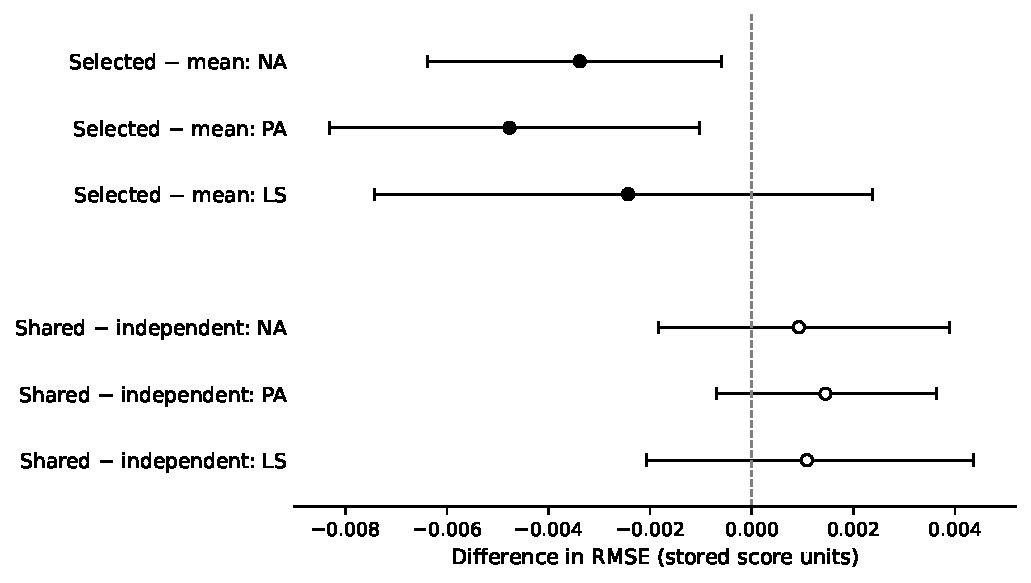
\includegraphics[width=\linewidth]{figures/paired_error.pdf}
\caption{Paired holdout RMSE differences for the two planned comparisons ($n=104$). Points are first-model-minus-second-model estimates; bars are pointwise 95\% intervals from 5,000 paired participant bootstrap resamples. Negative values favor the first model. The vertical line marks zero difference. These intervals are not adjusted for multiplicity; the six Holm-adjusted prediction-swap tests are reported separately in Table~\ref{tab:paired}.}\label{fig:paired}
\end{figure}
\FloatBarrier

\subsection{Contributions of linguistic categories}
The largest mean absolute development-set SHAP contributions differed across outcomes (Table~\ref{tab:shap}). Negative affect was led by \texttt{Sexual} (0.0041), \texttt{C10} (0.0040), and \texttt{C2} (0.0036); positive affect by \texttt{Sexual} (0.0045), \texttt{We} (0.0039), and \texttt{Family} (0.0030); and life satisfaction by \texttt{Family} (0.0061), \texttt{We} (0.0056), and \texttt{C10} (0.0052). These values describe the magnitude of contributions to fitted predictions in stored score units. The unmapped codes retain their literal labels, and absolute contributions supply no direction of association.

\begin{table}[!htbp]
\centering
\begingroup\singlespacing\fontsize{9.2}{11.32}\selectfont
\setlength{\tabcolsep}{3pt}
\caption{Three largest mean absolute TreeSHAP contributions per outcome}\label{tab:shap}
\begin{tabular}{@{}>{\raggedright\arraybackslash}p{0.16\linewidth}>{\raggedright\arraybackslash}p{0.12\linewidth}>{\raggedright\arraybackslash}p{0.32\linewidth}>{\raggedright\arraybackslash}p{0.28\linewidth}@{}}
\toprule
Outcome & Rank & Feature & Mean absolute SHAP \\
\midrule
NA & 1 & Sexual & 0.0041 \\
NA & 2 & C10$^{\dagger}$ & 0.0040 \\
NA & 3 & C2$^{\dagger}$ & 0.0036 \\
PA & 1 & Sexual & 0.0045 \\
PA & 2 & We & 0.0039 \\
PA & 3 & Family & 0.0030 \\
LS & 1 & Family & 0.0061 \\
LS & 2 & We & 0.0056 \\
LS & 3 & C10$^{\dagger}$ & 0.0052 \\
\bottomrule
\end{tabular}
\tabnote{NA = negative affect; PA = positive affect; LS = life satisfaction. Shared RF, development $n=933$. Values retain stored outcome units and use a tree-path-dependent background. $\dagger$ Unverified semantic mapping. Magnitude is not direction, statistical significance, or a causal effect.}
\endgroup
\end{table}


The holdout perturbation diagnostics produced small changes of mixed sign. For positive affect, permuting \texttt{Sexual}, the highest-ranked development feature, changed RMSE by only 0.000002 on average, with an across-shuffle SD of 0.000544. For life satisfaction, the mean changes were 0.001030 for \texttt{Family} and $-0.000935$ for \texttt{We}. Thus, prominence in development-set attribution did not consistently correspond to a deterioration in holdout error when a feature was shuffled. Supplementary Table S6 shows the mean and shuffle variability for every selected feature and outcome.

\subsection{Sensitivity analyses and exploratory extension}
Using the latest records yielded selected-model correlations of 0.259, 0.286, and 0.101 for negative affect, positive affect, and life satisfaction. Restricting the analysis to participants observed once retained 85 holdout participants and yielded correlations of 0.303, 0.301, and 0.173. Removing \texttt{ind} and the unmapped codes yielded correlations of 0.301, 0.268, and 0.125, with RMSEs of 0.165, 0.165, and 0.203. These handling choices altered point estimates while retaining the broad pattern of modest associations and limited score estimation (Supplementary Table S3). The repeated development-fold summaries are reported descriptively in Supplementary Table S4.

Exploratory optimization selected independent forests with a minimum leaf size of 60 and half the predictors considered at each split. Outer-fold macro normalized RMSE was 1.0006 for the selected procedure, 1.0001 for the fixed original shared forest, and 1.0007 for the mean baseline. The selected procedure's error was 0.044\% higher than the original forest's, failing the planned 1\% improvement heuristic. On the previously seen holdout, correlations were 0.245, 0.332, and 0.164, with RMSEs of 0.1661, 0.1645, and 0.2023. An exploratory positive-affect comparison with the mean gave Holm-adjusted $p=0.011$, whereas comparisons with the original forest all had adjusted $p=1.000$. These reused-holdout estimates are reported alongside the complete exploratory search in Supplementary Tables S7--S10 and do not replace the primary results.

\section{Discussion}
\subsection{What the language signal contributes to assessment}
The principal finding is a modest language--affect association that translates into only small gains in estimating questionnaire-derived scores. This adds a quantitative qualification to the proposed use of psycholinguistic categories for well-being assessment. In this sample, the selected model captured linear covariation with both affect outcomes, but most of the numerical prediction error remained after using the language features. Life satisfaction was estimated less precisely in terms of its correlation interval. The contribution is therefore an evaluation of the information retained by this representation and these learning procedures, with the size of the error improvement making the assessment claim more specific than a significance test alone.

The positive-affect comparison between the elastic net and selected forest makes this distinction concrete. A visibly larger correlation coexisted with essentially the same RMSE. Mathematically, positive rescaling and shifting of predictions can leave Pearson correlation unchanged while changing their distance from observed scores. Consequently, a model that tracks relative linear variation need not reproduce the level or spread of individual scores. Here, the small baseline-relative error differences are the relevant evidence for numerical estimation. Whether that magnitude is useful would depend on an intended decision, an interpretable score scale, and an acceptable error criterion; none was specified in this dataset.

The different outcome estimates raise a substantive hypothesis about what aggregate language categories represent. Affect-related expression may be more directly reflected in these categories than the standards people use to judge their lives as a whole. The distinction between affect and global life evaluation provides a conceptual reason to investigate this possibility \citep{diener1984,diener1985}. The present pattern, however, can also arise from differences in criterion reliability, the temporal match between text and questionnaires, or sampling variability. Because the outcome correlations were not directly contrasted and the administered measures were incompletely documented, the results support component-specific validation rather than a conclusion that affect is intrinsically more predictable. A design that holds language exposure and measurement quality constant across outcomes would discriminate these explanations more effectively.

\subsection{Representation, shared learning, and interpretation}
The limited gains from exploratory optimization focus attention on the information entering the models. Changing regularization, smoothness, or dimensionality while retaining the same aggregate feature matrix did not reduce nested development error relative to the original forest. This result gives little empirical support for continuing the tested forms of tuning on these inputs, while leaving representation and criterion quality as unresolved alternatives. Closed- and open-vocabulary approaches can capture different linguistic cues \citep{eichstaedt2021}, and the amount of language available per participant affects the basis for estimation \citep{kern2016}. A within-sample comparison of fixed categories with richer language representations, using identical time windows, criteria, and evaluation participants, would test whether category aggregation discards useful information. It would be more informative than attributing the present errors to model complexity alone.

The shared-output comparison provides a second boundary on the proposed approach. Correlated well-being outcomes supplied a rationale for borrowing information, but useful sharing requires compatible feature--outcome relationships. Common tree partitions impose a particular form of that compatibility \citep{caruana1997,kocev2007}. The shared forest's marginal development advantage and slightly higher holdout errors are consistent with effects small enough to be difficult to distinguish in this sample. They also leave open the possibility that useful linguistic relationships overlap only partly across components. Because independent models selected outcome-specific parameters and the shared model selected one common setting, the current estimates cannot isolate the effect of sharing itself. A more discriminating comparison would match the tuning opportunities and examine repeated, outcome-specific differences in a new sample.

The attribution results locate features used by the model, but the accompanying perturbation results place their psychological interpretation on a firmer empirical footing. The near-zero positive-affect error change after shuffling \texttt{Sexual} contrasts with its leading development attribution. Such a contrast may reflect redundant features, unstable fitted relationships, or limited sensitivity of a small holdout diagnostic; it does not identify which explanation applies. TreeSHAP summarizes contributions under a specified background definition \citep{lundberg2020}, whereas disrupting an algorithm input is distinct from intervening on the corresponding real-world behavior \citep{janzing2020}. The two analyses therefore answer complementary questions about the predictor, not whether talking about a topic changes well-being. Prediction and causal explanation require different evidential designs \citep{shmueli2010}.

A useful next step for categories such as \texttt{Family} and \texttt{We} is to recover their actual vocabulary and distinguish self-description, descriptions of others, quotations, and idiomatic uses in the source posts. Evidence that Chinese dictionary matches can diverge from contextual meaning makes this distinction consequential \citep{zhao2016}. If a category's predictive contribution persists after contextual verification and replicates in a new sample, it would support investigation of a more specific linguistic correlate. If the contribution disappears or shifts among correlated categories, the original ranking would be better understood as a property of the fitted representation. Unmapped codes require a verified dictionary mapping before this substantive investigation is possible.

\subsection{From a retrospective predictor to a measurement study}
Temporal alignment is the first design requirement for extending these findings toward monitoring. Language features here could include posts written after the questionnaire, so the observed associations combine an incompletely specified period of expression with an earlier report. A temporally ordered study would define the language window before the outcome assessment and retain posts needed to verify that cutoff. Earlier work predicting depression documentation from Facebook explicitly placed language before the relevant medical-record event \citep{eichstaedt2018}; the transferable lesson is this ordering, not equivalence between depression and well-being. Repeated, matched language windows and questionnaires would then permit separate tests of between-person differences and within-person changes. Those two uses should be evaluated as distinct targets.

The questionnaire criteria also need a documented measurement basis. Verifying the administered items, reporting period, and score transformation would make error interpretable and allow assessment of criterion reliability. PANAS permits different reporting periods \citep{watson1988}, while temporal stability and sensitivity to meaningful life changes are distinct considerations for the SWLS \citep{pavot1993}. Language estimates would need their own evidence on these properties. The wider validation design used by \citet{park2015} illustrates why agreement with a questionnaire can be complemented by other methods and temporal tests. For this study, the immediate priority is to establish what the stored scores mean and whether time-matched language adds dependable information about them.

The present sample supports a bounded evaluation rather than population-wide generalization. It was a convenience sample, the holdout contained 104 participants, and demographic information was unavailable for examining subgroup performance. Uncertainty intervals condition on the existing fitted models and partition. Overlapping cross-validation training samples also make fold variability an unsuitable substitute for an independent-sample confidence interval \citep{varoquaux2018}. Participant separation and fold-local preprocessing address important evaluation risks \citep{kapoor2023}, while an independently recruited sample is needed to assess transport across people, periods, or platforms. The primary procedures should be frozen before that evaluation, with precision and acceptable error specified for the intended use.

The available aggregates limited how precisely we could diagnose the observed errors. Missing item responses prevented reliability checks on the supplied criteria; missing posts prevented reconstruction of language windows and vocabulary coverage; and incomplete dictionary documentation restricted interpretation of several features. The planned record and feature sensitivities examined particular handling choices, but could not resolve these source-level uncertainties. Recovering those inputs would permit a targeted comparison of representation loss, criterion noise, and temporal mismatch. This is a more specific next research step than treating the small effects either as proof of a deployable instrument or as a general ceiling on language-based well-being assessment.

For a future assessment use, performance should be judged by the information the estimate adds to direct reports and by the consequences of its errors. A proposed application could, for example, evaluate whether a language estimate improves a prespecified research measurement task when direct assessments are infrequent; that benefit would need to be demonstrated in the intended setting. Individual decision utility, population representativeness, and meaningful error thresholds were not evaluated here. Consent, privacy, and participants' control over sensitive inferences are also design requirements, as emphasized in prior social-media health-prediction work \citep{eichstaedt2018}. The present results provide a benchmark for that development process and identify the evidence needed to decide whether further deployment-oriented work is warranted.

\section{Conclusion}
Aggregated psycholinguistic features from Weibo contained modest retrospective information about positive and negative affect, with small observed gains in score estimation over a training-mean baseline. The selected shared-output procedure did not establish an advantage over independent forests, and prominent development-set attributions had mixed holdout error contributions. These findings define a limited predictive benchmark for the available representation. Further instrument development should establish interpretable scoring and temporal alignment, then test accuracy, stability, and generalization for a specified measurement purpose.

\section{Declarations}
\subsection{Data and code availability}
Analysis code and aggregate results are available in a public project repository; the identifying repository address is provided on the separate title page. Participant-level records, original posts, fitted model objects, and individual predictions are not included in that public repository. The data custodian, access conditions, sharing authorization, dataset citation, and any anonymized review link or archival persistent identifier are TO BE COMPLETED BY AUTHORS. No access commitment is made on behalf of the original data owner.

\subsection{Ethics and author statements}
Approval and consent are reported from the original collection documentation and require confirmation for this secondary use. Author identities, contributions, funding, conflicts of interest, acknowledgments, and final approval are TO BE COMPLETED BY AUTHORS on the separate title page.

\subsection{Use of artificial intelligence}
According to the project records, OpenAI Codex assisted with the earlier analysis-code development and execution, literature retrieval, evidence checking, figure preparation, and drafting. ChatGPT assisted with the present manuscript restructuring, English and Chinese writing, targeted source checking, aggregate-result presentation, and document checks. These forms of assistance do not constitute human-author approval. Responsible authors must verify and approve the provenance, analyses, interpretation, references, and declarations before submission.

\FloatBarrier
\begin{thebibliography}{99}
\interlinepenalty=10000
\bibitem[Breiman(2001)]{breiman2001}
Breiman, L. (2001). Random forests. \emph{Machine Learning, 45}(1), 5--32. \url{https://doi.org/10.1023/A:1010933404324}

\bibitem[Caruana(1997)]{caruana1997}
Caruana, R. (1997). Multitask learning. \emph{Machine Learning, 28}(1), 41--75. \url{https://doi.org/10.1023/A:1007379606734}

\bibitem[Cawley \& Talbot(2010)]{cawley2010}
Cawley, G. C., \& Talbot, N. L. C. (2010). On over-fitting in model selection and subsequent selection bias in performance evaluation. \emph{Journal of Machine Learning Research, 11}(70), 2079--2107. \url{https://jmlr.org/papers/v11/cawley10a.html}

\bibitem[Diener(1984)]{diener1984}
Diener, E. (1984). Subjective well-being. \emph{Psychological Bulletin, 95}(3), 542--575. \url{https://doi.org/10.1037/0033-2909.95.3.542}

\bibitem[Diener et al.(1985)]{diener1985}
Diener, E., Emmons, R. A., Larsen, R. J., \& Griffin, S. (1985). The satisfaction with life scale. \emph{Journal of Personality Assessment, 49}(1), 71--75. \url{https://doi.org/10.1207/s15327752jpa4901_13}

\bibitem[Diener et al.(2018)]{diener2018}
Diener, E., Lucas, R. E., \& Oishi, S. (2018). Advances and open questions in the science of subjective well-being. \emph{Collabra: Psychology, 4}(1), 15. \url{https://doi.org/10.1525/collabra.115}

\bibitem[Eichstaedt et al.(2021)]{eichstaedt2021}
Eichstaedt, J. C., Kern, M. L., Yaden, D. B., Schwartz, H. A., Giorgi, S., Park, G., Hagan, C. A., Tobolsky, V. A., Smith, L. K., Buffone, A., Iwry, J., Seligman, M. E. P., \& Ungar, L. H. (2021). Closed- and open-vocabulary approaches to text analysis: A review, quantitative comparison, and recommendations. \emph{Psychological Methods, 26}(4), 398--427. \url{https://doi.org/10.1037/met0000349}

\bibitem[Eichstaedt et al.(2018)]{eichstaedt2018}
Eichstaedt, J. C., Smith, R. J., Merchant, R. M., Ungar, L. H., Crutchley, P., Preoţiuc-Pietro, D., Asch, D. A., \& Schwartz, H. A. (2018). Facebook language predicts depression in medical records. \emph{Proceedings of the National Academy of Sciences, 115}(44), 11203--11208. \url{https://doi.org/10.1073/pnas.1802331115}

\bibitem[Geurts et al.(2006)]{geurts2006}
Geurts, P., Ernst, D., \& Wehenkel, L. (2006). Extremely randomized trees. \emph{Machine Learning, 63}(1), 3--42. \url{https://doi.org/10.1007/s10994-006-6226-1}

\bibitem[Jaidka et al.(2020)]{jaidka2020}
Jaidka, K., Giorgi, S., Schwartz, H. A., Kern, M. L., Ungar, L. H., \& Eichstaedt, J. C. (2020). Estimating geographic subjective well-being from Twitter: A comparison of dictionary and data-driven language methods. \emph{Proceedings of the National Academy of Sciences, 117}(19), 10165--10171. \url{https://doi.org/10.1073/pnas.1906364117}

\bibitem[Janzing et al.(2020)]{janzing2020}
Janzing, D., Minorics, L., \& Blöbaum, P. (2020). Feature relevance quantification in explainable AI: A causal problem. In S. Chiappa \& R. Calandra (Eds.), \emph{Proceedings of the Twenty Third International Conference on Artificial Intelligence and Statistics} (Vol. 108, pp. 2907--2916). PMLR. \url{https://proceedings.mlr.press/v108/janzing20a.html}

\bibitem[Kapoor \& Narayanan(2023)]{kapoor2023}
Kapoor, S., \& Narayanan, A. (2023). Leakage and the reproducibility crisis in machine-learning-based science. \emph{Patterns, 4}(9), 100804. \url{https://doi.org/10.1016/j.patter.2023.100804}

\bibitem[Kern et al.(2016)]{kern2016}
Kern, M. L., Park, G., Eichstaedt, J. C., Schwartz, H. A., Sap, M., Smith, L. K., \& Ungar, L. H. (2016). Gaining insights from social media language: Methodologies and challenges. \emph{Psychological Methods, 21}(4), 507--525. \url{https://doi.org/10.1037/met0000091}

\bibitem[Kocev et al.(2007)]{kocev2007}
Kocev, D., Vens, C., Struyf, J., \& Džeroski, S. (2007). Ensembles of multi-objective decision trees. In J. N. Kok, J. Koronacki, R. López de Mántaras, S. Matwin, D. Mladenič, \& A. Skowron (Eds.), \emph{Machine Learning: ECML 2007} (Vol. 4701, pp. 624--631). Springer Berlin Heidelberg. \url{https://doi.org/10.1007/978-3-540-74958-5_61}

\bibitem[Lundberg et al.(2020)]{lundberg2020}
Lundberg, S. M., Erion, G., Chen, H., DeGrave, A., Prutkin, J. M., Nair, B., Katz, R., Himmelfarb, J., Bansal, N., \& Lee, S.-I. (2020). From local explanations to global understanding with explainable AI for trees. \emph{Nature Machine Intelligence, 2}(1), 56--67. \url{https://doi.org/10.1038/s42256-019-0138-9}

\bibitem[Park et al.(2015)]{park2015}
Park, G., Schwartz, H. A., Eichstaedt, J. C., Kern, M. L., Kosinski, M., Stillwell, D. J., Ungar, L. H., \& Seligman, M. E. P. (2015). Automatic personality assessment through social media language. \emph{Journal of Personality and Social Psychology, 108}(6), 934--952. \url{https://doi.org/10.1037/pspp0000020}

\bibitem[Pavot \& Diener(1993)]{pavot1993}
Pavot, W., \& Diener, E. (1993). Review of the Satisfaction With Life Scale. \emph{Psychological Assessment, 5}(2), 164--172. \url{https://doi.org/10.1037/1040-3590.5.2.164}

\bibitem[Shmueli(2010)]{shmueli2010}
Shmueli, G. (2010). To explain or to predict? \emph{Statistical Science, 25}(3), 289--310. \url{https://doi.org/10.1214/10-STS330}

\bibitem[Tausczik \& Pennebaker(2010)]{tausczik2010}
Tausczik, Y. R., \& Pennebaker, J. W. (2010). The psychological meaning of words: LIWC and computerized text analysis methods. \emph{Journal of Language and Social Psychology, 29}(1), 24--54. \url{https://doi.org/10.1177/0261927X09351676}

\bibitem[Varoquaux(2018)]{varoquaux2018}
Varoquaux, G. (2018). Cross-validation failure: Small sample sizes lead to large error bars. \emph{NeuroImage, 180}, 68--77. \url{https://doi.org/10.1016/j.neuroimage.2017.06.061}

\bibitem[Watson et al.(1988)]{watson1988}
Watson, D., Clark, L. A., \& Tellegen, A. (1988). Development and validation of brief measures of positive and negative affect: The PANAS scales. \emph{Journal of Personality and Social Psychology, 54}(6), 1063--1070. \url{https://doi.org/10.1037/0022-3514.54.6.1063}

\bibitem[Yarkoni \& Westfall(2017)]{yarkoni2017}
Yarkoni, T., \& Westfall, J. (2017). Choosing prediction over explanation in psychology: Lessons from machine learning. \emph{Perspectives on Psychological Science, 12}(6), 1100--1122. \url{https://doi.org/10.1177/1745691617693393}

\bibitem[Zhao et al.(2016)]{zhao2016}
Zhao, N., Jiao, D., Bai, S., \& Zhu, T. (2016). Evaluating the validity of simplified Chinese version of LIWC in detecting psychological expressions in short texts on social network services. \emph{PLOS ONE, 11}(6), e0157947. \url{https://doi.org/10.1371/journal.pone.0157947}

\end{thebibliography}

\end{document}
